% Options for packages loaded elsewhere
\PassOptionsToPackage{unicode}{hyperref}
\PassOptionsToPackage{hyphens}{url}
\PassOptionsToPackage{dvipsnames,svgnames,x11names}{xcolor}
\documentclass[
  spanish,
  10pt,
  a4paper,
]{article}
\usepackage{xcolor}
\usepackage[top=22mm,bottom=22mm,left=22mm,right=22mm]{geometry}
\usepackage{amsmath,amssymb}
\setcounter{secnumdepth}{-\maxdimen} % remove section numbering
\usepackage{iftex}
\ifPDFTeX
  \usepackage[T1]{fontenc}
  \usepackage[utf8]{inputenc}
  \usepackage{textcomp} % provide euro and other symbols
\else % if luatex or xetex
  \usepackage{unicode-math} % this also loads fontspec
  \defaultfontfeatures{Scale=MatchLowercase}
  \defaultfontfeatures[\rmfamily]{Ligatures=TeX,Scale=1}
\fi
\usepackage{lmodern}
\ifPDFTeX\else
  % xetex/luatex font selection
\fi
% Use upquote if available, for straight quotes in verbatim environments
\IfFileExists{upquote.sty}{\usepackage{upquote}}{}
\IfFileExists{microtype.sty}{% use microtype if available
  \usepackage[]{microtype}
  \UseMicrotypeSet[protrusion]{basicmath} % disable protrusion for tt fonts
}{}
\usepackage{setspace}
\makeatletter
\@ifundefined{KOMAClassName}{% if non-KOMA class
  \IfFileExists{parskip.sty}{%
    \usepackage{parskip}
  }{% else
    \setlength{\parindent}{0pt}
    \setlength{\parskip}{6pt plus 2pt minus 1pt}}
}{% if KOMA class
  \KOMAoptions{parskip=half}}
\makeatother
\usepackage{longtable,booktabs,array}
\newcounter{none} % for unnumbered tables
\usepackage{calc} % for calculating minipage widths
% Correct order of tables after \paragraph or \subparagraph
\usepackage{etoolbox}
\makeatletter
\patchcmd\longtable{\par}{\if@noskipsec\mbox{}\fi\par}{}{}
\makeatother
% Allow footnotes in longtable head/foot
\IfFileExists{footnotehyper.sty}{\usepackage{footnotehyper}}{\usepackage{footnote}}
\makesavenoteenv{longtable}
\usepackage{graphicx}
\makeatletter
\newsavebox\pandoc@box
\newcommand*\pandocbounded[1]{% scales image to fit in text height/width
  \sbox\pandoc@box{#1}%
  \Gscale@div\@tempa{\textheight}{\dimexpr\ht\pandoc@box+\dp\pandoc@box\relax}%
  \Gscale@div\@tempb{\linewidth}{\wd\pandoc@box}%
  \ifdim\@tempb\p@<\@tempa\p@\let\@tempa\@tempb\fi% select the smaller of both
  \ifdim\@tempa\p@<\p@\scalebox{\@tempa}{\usebox\pandoc@box}%
  \else\usebox{\pandoc@box}%
  \fi%
}
% Set default figure placement to htbp
\def\fps@figure{htbp}
\makeatother
\ifLuaTeX
\usepackage[bidi=basic,shorthands=off]{babel}
\else
\usepackage[bidi=default,shorthands=off]{babel}
\fi
\ifLuaTeX
  \usepackage{selnolig} % disable illegal ligatures
\fi
\setlength{\emergencystretch}{3em} % prevent overfull lines
\providecommand{\tightlist}{%
  \setlength{\itemsep}{0pt}\setlength{\parskip}{0pt}}

\usepackage{amsmath,amssymb,mathtools}
\usepackage{microtype}
\usepackage{fancyhdr}
\usepackage{needspace}
\usepackage{etoolbox}
\usepackage{float}
\usepackage{caption}
\captionsetup{font=small,labelformat=empty,skip=7pt}
\floatplacement{figure}{H}
\definecolor{DocBlue}{HTML}{173F57}
\definecolor{DocGray}{HTML}{52616C}
\pagestyle{fancy}
\fancyhf{}
\fancyhead[L]{\small\sffamily\color{DocGray} pySNSPD | Desarrollo del modelo}
\fancyhead[R]{\small\sffamily\color{DocGray} Revisión 0.4}
\fancyfoot[L]{\small\sffamily\color{DocGray} 9 de septiembre de 2026}
\fancyfoot[R]{\small\sffamily\thepage}
\setlength{\headheight}{15pt}
\setlength{\emergencystretch}{2em}
\setlength{\parskip}{5pt plus 1pt}
\setlength{\parindent}{0pt}
\widowpenalty=10000
\clubpenalty=10000
\displaywidowpenalty=10000
\predisplaypenalty=10000
\renewcommand{\arraystretch}{1.16}
\AtBeginEnvironment{longtable}{\small}
\pretocmd{\section}{\Needspace{6\baselineskip}}{}{}
\pretocmd{\subsection}{\Needspace{5\baselineskip}}{}{}
\AtBeginDocument{\hypersetup{colorlinks=true,linkcolor=DocBlue,urlcolor=DocBlue}}
\allowdisplaybreaks[1]
\usepackage{bookmark}
\IfFileExists{xurl.sty}{\usepackage{xurl}}{} % add URL line breaks if available
\urlstyle{same}
\hypersetup{
  pdftitle={C. Condensado{,} corriente y señal},
  pdflang={es},
  colorlinks=true,
  linkcolor={Maroon},
  filecolor={Maroon},
  citecolor={Blue},
  urlcolor={Blue},
  pdfcreator={LaTeX via pandoc}}

\title{C. Condensado, corriente y señal}
\usepackage{etoolbox}
\makeatletter
\providecommand{\subtitle}[1]{% add subtitle to \maketitle
  \apptocmd{\@title}{\par {\large #1 \par}}{}{}
}
\makeatother
\subtitle{Auditoría y contrato experimental · Documento 3 de 5}
\author{}
\date{9 de septiembre de 2026 · Revisión 0.4}

\begin{document}
\maketitle

{
\setcounter{tocdepth}{1}
\tableofcontents
}
\setstretch{1.07}
\newpage

\section{C.0. De la ecuación de la memoria al cambio de
fuerza}\label{c.0.-de-la-ecuaciuxf3n-de-la-memoria-al-cambio-de-fuerza}

\textbf{Resultado de la auditoría.} La sustitución de la fuerza local
está bien definida cuando la amplitud es distinta de cero y el espectro
local es válido. La formulación polar de 0.3, por sí sola, no cierra la
evolución de un núcleo donde \(\Delta=0\). Las pruebas nuevas muestran
que una energía casi invariable puede acompañar fuerzas de núcleo muy
diferentes; además, la extensión finita puede perder difusión de fase
estable a gradientes elevados. Por eso se define aquí \textbf{un solo
candidato experimental con una escala de núcleo finita y un dominio de
admisión explícito}, conservativo y verificable, cuya promoción a
producción queda pendiente. La elección de movilidad KWT sigue siendo
una hipótesis dinámica independiente del funcional estático.

\subsection{C.0.1. Resultado complejo que se
conserva}\label{c.0.1.-resultado-complejo-que-se-conserva}

La ecuación final de la memoria, con \(\Delta=|\Delta|e^{i\theta}\),
\(e>0\) y \(\mathbf A=0\), es

\[
\begin{aligned}
\frac{\pi\hbar}{8k_BT_c}\left[
\left(\partial_t+\frac{2ie}{\hbar}\phi\right)\Delta
+\frac{2\tau_{sc}^2}{\hbar^2}\partial_t|\Delta|^2\,\Delta
\right]
={}&R_{\rm KWT}\Bigg\{
\xi_{\rm mod}^2\nabla^2\Delta\\
&+\left[1-\frac{T_e}{T_c}-\frac{|\Delta|^2}{\Delta_{\rm mod}^2}\right]\Delta\\
&+i\frac{\hbar eD}{\sigma_n\sqrt2\sqrt{1+T_e/T_c}}
\left(\nabla\!\cdot\mathbf j_s^{\rm Us}-\nabla\!\cdot\mathbf j_s^{\rm GL}\right)
\frac{\Delta}{|\Delta|^2}\Bigg\}.
\end{aligned}\tag{C.1}
\]

Es la ecuación (C.3), p.~impresa 121 / PDF 152, de la copia cotejada de
la memoria {[}M{]}, construida desde Allmaras {[}A, ec. 3.24{]}. Se
conserva su forma compleja y su término temporal no lineal, empleados
por la actualización numérica estable. Para campos magnéticos resueltos,
el laplaciano pasa a ser covariante. Los coeficientes de referencia son

\[
\begin{gathered}
\tau_0=\frac{\pi\hbar}{8k_BT_c},\qquad
R_{\rm KWT}=\sqrt{1+4|\Delta|^2\tau_{sc}^2/\hbar^2},\\
\xi_{\rm mod}^2(T_e)=\frac{\pi\hbar D}{4\sqrt2 k_BT_c\sqrt{1+T_e/T_c}},\\
\Delta_{\rm mod}^2(T_e)=\frac{\Delta_0^2}{1-T_e/T_c}
\tanh^2\!\left[1.74\sqrt{T_c/T_e-1}\right],\quad 0<T_e<T_c,\\
\mathbf j_s^{\rm GL}=\frac{\pi\sigma_n}{4ek_BT_c}|\Delta|^2\mathbf q,
\qquad \mathbf q=\nabla\theta-\frac{2e}{\hbar}\mathbf A.
\end{gathered}\tag{C.2}
\]

\(\Delta_{\rm mod}\) es un coeficiente, no la amplitud instantánea. Su
extensión histórica por encima de \(T_c\) no se necesita en la nueva
fuerza microscópica; no se modifica el solver antiguo. En C.1, la
corriente Usadel de la memoria recibe \(T_e,|\Delta|,q\)
independientemente: no se vuelve a imponer la ecuación de gap durante el
transitorio.

Multiplicar el corchete temporal por \(e^{-i\theta}\) muestra qué
conserva la reformulación:

\[
e^{-i\theta}\left[D_t\Delta+
\frac{2\tau_{sc}^2}{\hbar^2}\partial_t|\Delta|^2\Delta\right]
=R_{\rm KWT}^2\partial_t|\Delta|
+i|\Delta|\left(\dot\theta+\frac{2e}{\hbar}\phi\right),
\quad D_t=\partial_t+\frac{2ie}{\hbar}\phi.
\tag{C.3}
\]

Después de dividir C.1 por \(R_{\rm KWT}\), amplitud y fase llevan los
factores \(R_{\rm KWT}\) y \(1/R_{\rm KWT}\). Eliminar el término
\(\partial_t|\Delta|^2\Delta\) cambiaría esa dinámica.

\subsection{\texorpdfstring{C.0.2. De dónde sale exactamente el término
en
\(q^2\)}{C.0.2. De dónde sale exactamente el término en q\^{}2}}\label{c.0.2.-de-duxf3nde-sale-exactamente-el-tuxe9rmino-en-q2}

El operador espacial actúa tanto sobre la longitud como sobre el ángulo
de la variable compleja. Para verlo, se quita localmente la fase,
manteniendo \(|\Delta|>0\):

\[
\begin{aligned}
e^{-i\theta}\left(\nabla-\frac{2ie}{\hbar}\mathbf A\right)^2\Delta
&=(\nabla+i\mathbf q)^2|\Delta|\\
&=\nabla^2|\Delta|-|\Delta|q^2
+i\left(2\nabla|\Delta|\cdot\mathbf q+|\Delta|\nabla\cdot\mathbf q\right).
\end{aligned}\tag{C.4}
\]

En una dimensión, la pieza decisiva es
\(\partial_x(iq|\Delta|)+iq\,\partial_x|\Delta|\): contiene
\(i|\Delta|q'+2iq|\Delta|'-q^2|\Delta|\). El signo menos procede de
\(i^2=-1\). Aunque la amplitud sea constante, una fase que gira
espacialmente hace variar el campo complejo y cuesta energía. La
ecuación de amplitud conserva esa influencia como
\(-\xi_{\rm mod}^2q^2|\Delta|\).

La parte imaginaria del gradiente genera primero la divergencia GL
auxiliar. Con \(\sigma_n,T_c\) constantes,

\[
\begin{gathered}
\nabla\cdot\mathbf j_s^{\rm GL}
=\frac{\pi\sigma_n|\Delta|}{4ek_BT_c}
\left(2\nabla|\Delta|\cdot\mathbf q+|\Delta|\nabla\cdot\mathbf q\right),\\
\nabla\cdot\mathbf j_s^{\rm GL}
+\nabla\cdot(\mathbf j_s^{\rm Us}-\mathbf j_s^{\rm GL})
=\nabla\cdot\mathbf j_s^{\rm Us}.
\end{gathered}\tag{C.5}
\]

Esta cancelación explica la corrección de Vodolazov--Allmaras {[}V,
p.~11; M, anexo C.2{]}. No aparecen dos corrientes físicas sumadas. La
parte real de C.1, después de quitar su fase, queda

\[
\xi_{\rm mod}^2\nabla^2|\Delta|
+\left[1-\frac{T_e}{T_c}-\frac{|\Delta|^2}{\Delta_{\rm mod}^2}
-\xi_{\rm mod}^2q^2\right]|\Delta|.
\tag{C.6}
\]

\subsection{C.0.3. Qué se reemplaza y qué no se debe contar dos
veces}\label{c.0.3.-quuxe9-se-reemplaza-y-quuxe9-no-se-debe-contar-dos-veces}

A obtiene una fuerza microscópica \(X_{|\Delta|}\) que \textbf{ya
depende del superflujo}, porque el espectro depende de
\(\Gamma=\hbar Dq^2/2\). En el cierre polar exterior de 0.3, el
reemplazo correcto era

\[
\left[1-\frac{T_e}{T_c}-\frac{|\Delta|^2}{\Delta_{\rm mod}^2}
-\xi_{\rm mod}^2q^2\right]|\Delta|
\longrightarrow-\frac{X_{|\Delta|}}{2A_0},\qquad
A_0=N_0\sqrt{\frac{1+T_{\rm mob}/T_c}{2}}.
\tag{C.7}
\]

Se reemplaza el \textbf{corchete completo}, incluido su término de
depareamiento. Conservar además \(-\xi_{\rm mod}^2q^2|\Delta|\) junto a
\(X_{|\Delta|}\) duplicaría ese efecto. Otra comprobación es energética:
si el funcional uniforme ya depende de \(q\), añadir por separado
\(K_0|\Delta|^2q^2\) añade otra energía de superflujo. La temperatura de
movilidad \(T_{\rm mob}\) se fija en la sección C.5; cuando coincide con
\(T_e\) recupera el coeficiente de referencia.

Esta observación valida la contabilidad de la sustitución; no demuestra
que una expresión escrita mediante \(\nabla\arg\Delta\) siga siendo
diferenciable en un cero. La revisión 0.4 conserva el cambio de fuerza
en el exterior y deriva \textbf{toda} la ecuación de una extensión
cartesiana finita. Sus términos adicionales se fijan en C.1--C.2 y no se
eliminan por parecer pequeños.

\section{C.1. Un funcional único que también define el
núcleo}\label{c.1.-un-funcional-uxfanico-que-tambiuxe9n-define-el-nuxfacleo}

\subsection{C.1.1. Variables y escala finita
elegida}\label{c.1.1.-variables-y-escala-finita-elegida}

Definimos las cantidades regulares

\[
\begin{gathered}
\mathcal D_i=\partial_i-\frac{2ie}{\hbar}A_i,\qquad
\rho_\Delta=|\Delta|^2,\qquad
P_i=\operatorname{Im}(\Delta^*\mathcal D_i\Delta),\\
s_\delta=\rho_\Delta+\delta^2,\qquad
\mathbf q_\delta=\frac{\mathbf P}{s_\delta},\qquad
m=\frac{\rho_\Delta}{s_\delta},\qquad
\delta=0.10\Delta_0,\quad\Delta_0=\pi e^{-\gamma_E}k_BT_c.
\end{gathered}\tag{C.8}
\]

\(\rho_\Delta\) es el cuadrado de la amplitud y no la DOS electrónica
\(\rho(E)\) de B. \(\mathbf P\) mide el flujo covariante del campo
complejo antes de multiplicarlo por una rigidez. \(\mathbf q_\delta\) es
el argumento del \textbf{espectro efectivo del prototipo}, distinto de
\(\nabla\theta-(2e/\hbar)\mathbf A\) cerca del núcleo. Cuando
\(|\Delta|\gg\delta\), \(m\to1\) y se recupera ese argumento exterior.
En un cero, \(\mathbf P=0\) y \(\mathbf q_\delta=0\) sin dividir por la
amplitud.

El valor \(0.10\Delta_0\) fija una referencia experimental reproducible,
situada entre los controles \(0.05\Delta_0\) y \(0.20\Delta_0\).
\textbf{No es un parámetro material calibrado ni un resultado convergido
respecto del núcleo.} La prueba C.7 muestra por qué no se acepta todavía
una predicción de nucleación con esa elección. No se toma el límite
\(\delta\to0\) como parte del modelo.

\subsection{C.1.2. Energía y espectro compartidos con
B}\label{c.1.2.-energuxeda-y-espectro-compartidos-con-b}

El único funcional dinámico es

\[
\begin{gathered}
\mathcal U_\delta[\Delta,\mathbf A;p]=\int_{\mathcal V}e_\delta\,dV,\\
e_\delta=u_e(|\Delta|,\mathbf q_\delta;p)
+K_0\left[\sum_i|\mathcal D_i\Delta|^2
-\rho_\Delta|\mathbf q_\delta|^2\right],\\
K_0=\frac{\pi N_0\hbar D}{8k_BT_c},\qquad
u_e=U_{\rm vac}(|\Delta|,q_\delta)
+4N_0\int_0^\infty E(x;|\Delta|,q_\delta)p(x)\,dx.
\end{gathered}\tag{C.9}
\]

B define el espectro, la coordenada \(x\) y las ocupaciones \(p\). Al
variar \(\Delta\) se mantienen fijas las ocupaciones de esos estados. El
término adicional no depende explícitamente de \(p\): \textbf{las
colisiones de B y el balance de C usan exactamente la misma energía
\(E(x;|\Delta|,q_\delta)\)}. No se mezclan un espectro de corriente y
otro de calentamiento.

La contribución espacial es no negativa, pues

\[
|\mathbf P|^2\leq\rho_\Delta\sum_i|\mathcal D_i\Delta|^2
\quad\Longrightarrow\quad
\sum_i|\mathcal D_i\Delta|^2-\rho_\Delta q_\delta^2
\geq(1-m^2)\sum_i|\mathcal D_i\Delta|^2\geq0.
\tag{C.10}
\]

En el exterior, C.9 tiende a
\(u_e(|\Delta|,q;p)+K_0|\nabla|\Delta||^2\). En el núcleo recupera el
gradiente complejo completo. Esta construcción cierra una energía
efectiva; la desigualdad C.10 no demuestra que reproduzca la energía
espacial de Usadel ni la barrera de entrada de un vórtice.

Para una población térmica se utiliza el correspondiente funcional libre
\(\mathcal F_\delta=\mathcal U_\delta-Ts_e\), variado a temperatura
fija. No se emplea \(\mathcal F_\delta(T_E)\) para sustituir una
población no térmica durante la evolución.

\section{C.2. Fuerza, corriente y movilidad en variables
complejas}\label{c.2.-fuerza-corriente-y-movilidad-en-variables-complejas}

\subsection{C.2.1. Derivar antes de
discretizar}\label{c.2.1.-derivar-antes-de-discretizar}

B entrega las derivadas del término electrónico local, \(X_{|\Delta|}\)
y \(\boldsymbol\Pi=\partial_{\mathbf q_\delta}u_e\). Son entradas
constitutivas; \(2e\boldsymbol\Pi/\hbar\) no es, por sí solo, la
corriente espacial del núcleo regularizado. Definimos

\[
\begin{gathered}
\mathbf V_\delta=\frac{\boldsymbol\Pi-2K_0\rho_\Delta\mathbf q_\delta}{s_\delta},\\
h_\rho=\frac{X_{|\Delta|}}{2|\Delta|}
-\frac{\boldsymbol\Pi\cdot\mathbf q_\delta}{s_\delta}
+K_0q_\delta^2(2m-1),\\
\left.\delta e_\delta\right|_p
=h_\rho\,\delta\rho_\Delta+\mathbf V_\delta\cdot\delta\mathbf P
+K_0\,\delta\!\left(\sum_i|\mathcal D_i\Delta|^2\right).
\end{gathered}\tag{C.11}
\]

La última fila usa
\(\delta\mathbf q_\delta=\delta\mathbf P/s_\delta-\mathbf q_\delta\delta\rho_\Delta/s_\delta\).
Sustituir las variaciones de \(\rho_\Delta\) y \(\mathbf P\), e integrar
los gradientes por partes, da

\[
\mathscr F_\delta:=\frac{\delta\mathcal U_\delta}{\delta\Delta^*}
=h_\rho\Delta-K_0\mathcal D_i\mathcal D_i\Delta
-i\mathbf V_\delta\cdot\boldsymbol{\mathcal D}\Delta
-\frac{i}{2}(\nabla\cdot\mathbf V_\delta)\Delta.
\tag{C.12}
\]

Se suma sobre el índice espacial \(i\). El factor \(1/2\) procede de la
derivada compleja de Wirtinger: la fuerza en las dos componentes reales
es
\(2(\operatorname{Re}\mathscr F_\delta,\operatorname{Im}\mathscr F_\delta)\).
Puede verificarse escribiendo la variación en función de
\(\delta\rho_\Delta\), \(\delta\mathbf P\) y
\(\delta\sum_i|\mathcal D_i\Delta|^2\), e integrando el último término
por partes.

La definición primaria es la primera variación de C.9. En un cero se
evalúa el producto \([X_{|\Delta|}/|\Delta|]\Delta\) mediante su límite
continuo, nulo cuando \(X=O(|\Delta|\ln|\Delta|)\), y no se calcula
\(h_\rho\) como una división aislada por cero. Se conserva una derivada
espacial de esa misma energía; un recorte independiente de \(q\),
corriente o fuerza dejaría de implementar C.9.

La corriente física se obtiene al variar el potencial vectorial:

\[
\begin{aligned}
\mathbf j_{s,\delta}
&=-\frac{\delta\mathcal U_\delta}{\delta\mathbf A}
=\frac{2e}{\hbar}\left(2K_0\mathbf P+\rho_\Delta\mathbf V_\delta\right)\\
&=\frac{2e}{\hbar}\left[m\boldsymbol\Pi
+2K_0(1-m^2)\mathbf P\right].
\end{aligned}\tag{C.13}
\]

Esta misma corriente entra en Poisson, trabajo eléctrico y circuito. En
\(\Delta=0\) vale cero para gradientes finitos. Lejos del núcleo
recupera la corriente espectral. Mantener sólo
\(2e\boldsymbol\Pi/\hbar\) en la ecuación eléctrica sería una mezcla de
cierres, aunque ambas expresiones fueran próximas en la mayor parte de
la película.

\subsection{C.2.2. Se conserva la forma temporal estable de la
memoria}\label{c.2.2.-se-conserva-la-forma-temporal-estable-de-la-memoria}

La ley elegida es

\[
\frac{A_0\tau_0}{R}\left[
D_t\Delta+\frac{2\tau_\psi^2}{\hbar^2}\partial_t\rho_\Delta\,\Delta
\right]=-\mathscr F_\delta,
\qquad R=\sqrt{1+4\rho_\Delta\tau_\psi^2/\hbar^2}.
\tag{C.14}
\]

C.14 conserva la estructura compleja de C.1. Cambian la fuerza y la
corriente constitutivas; \(\tau_\psi\) se declara como movilidad
efectiva. La evolución de poblaciones de B no demuestra que esta
movilidad represente correctamente los grados microscópicos eliminados.

La ausencia de una singularidad temporal se ve en las dos componentes
\(\mathbf z=(\operatorname{Re}\Delta,\operatorname{Im}\Delta)\) y
\(\mathbf v\) correspondientes a \(D_t\Delta\):

\[
\begin{gathered}
\boldsymbol\Gamma\,\mathbf v=-\frac{\delta\mathcal U_\delta}{\delta\mathbf z},\qquad
\boldsymbol\Gamma=\frac{2A_0\tau_0}{R}
\left[\mathbf1+\frac{4\tau_\psi^2}{\hbar^2}\mathbf z\mathbf z^T\right],\\
\Gamma_{\parallel}=2A_0\tau_0R,\qquad
\Gamma_{\perp}=2A_0\tau_0/R>0.
\end{gathered}\tag{C.15}
\]

En un cero, ambas direcciones tienen el mismo coeficiente finito
\(2A_0\tau_0\). No hace falta definir allí una fase. La potencia
disipada por esta ley es

\[
Q_\Delta=\frac{2A_0\tau_0}{R}
\left[|D_t\Delta|^2+\frac{\tau_\psi^2}{\hbar^2}(\partial_t\rho_\Delta)^2\right]
=\mathbf v^T\boldsymbol\Gamma\mathbf v\geq0.
\tag{C.16}
\]

\textbf{Prueba nueva.} En un campo periódico con 128 nodos y dos ceros
exactos se compararon C.12 y C.13 con variaciones independientes de
cinco puntos del funcional libre térmico a temperatura fija. Los errores
relativos escalados fueron \(4.34\times10^{-11}\) y
\(7.40\times10^{-12}\). Una transformación de calibre cambió ese
funcional en \(2.22\times10^{-16}\) relativo. La igualdad entre potencia
perdida y C.16 tuvo residuo relativo \(1.78\times10^{-16}\). Esto
verifica la implementación de la primera variación en su especialización
térmica y su contabilidad, no la fidelidad física del núcleo. El balance
con ocupaciones no térmicas se prueba por separado en C.10.

\section{C.3. Conservación de corriente y
potencial}\label{c.3.-conservaciuxf3n-de-corriente-y-potencial}

En la aproximación cuasineutra seleccionada,

\[
\begin{gathered}
\mathbf E=-\nabla\phi-\partial_t\mathbf A,\qquad
\mathbf j_n=\sigma_n\mathbf E,\qquad
\nabla\cdot(\mathbf j_{s,\delta}+\mathbf j_n)=0,\\
\mathbf A=0:\qquad \sigma_n\nabla^2\phi=\nabla\cdot\mathbf j_{s,\delta}.
\end{gathered}\tag{C.17}
\]

\(\sigma_n\) es constante en el material de referencia. Se omiten el
campo magnético propio y el desequilibrio espectral de carga; la fase
compleja todavía puede formar vórtices y deslizamientos. La ecuación
eléctrica no usa la corriente GL auxiliar ni una segunda corriente
Usadel añadida. La corriente normal proporciona la potencia
\(\sigma_nE^2\) que se entrega una sola vez a B.

\section{C.4. Balance energético que incluye la extensión de
núcleo}\label{c.4.-balance-energuxe9tico-que-incluye-la-extensiuxf3n-de-nuxfacleo}

\subsection{C.4.1. Identidad local de
trabajo}\label{c.4.1.-identidad-local-de-trabajo}

La integración por partes que produjo C.12 también determina el flujo de
trabajo del condensado. En notación compleja,

\[
Z_i=2K_0\mathcal D_i\Delta+iV_{\delta,i}\Delta,
\qquad J_{{\rm tr},i}=\operatorname{Re}(Z_i^*D_t\Delta).
\tag{C.18}
\]

La derivada covariante cumple
\([D_t,\mathcal D_i]\Delta=(2ie/\hbar)E_i\Delta\). Aplicando la regla de
la cadena a C.9, a ocupaciones fijas, e integrando localmente por
partes,

\[
\left.\partial_te_\delta\right|_{\rm campos}
=2\operatorname{Re}(\mathscr F_\delta^*D_t\Delta)
+\mathbf j_{s,\delta}\cdot\mathbf E+\nabla\cdot\mathbf J_{\rm tr}
=-Q_\Delta+\mathbf j_{s,\delta}\cdot\mathbf E+\nabla\cdot\mathbf J_{\rm tr}.
\tag{C.19}
\]

Por otra parte, B entrega el momento energético de la evolución de
ocupaciones:

\[
4N_0\int E\dot p\,dx=-\nabla\cdot\mathbf Q_e
+\sigma_nE^2+Q_\Delta-P_{e\text{-ph}}+S_{\gamma,e}^{(E)}.
\tag{C.20}
\]

Sumar ambas identidades cancela \(Q_\Delta\). Al incluir la energía
fonónica,

\[
\partial_t(e_\delta+u_{\rm ph})
=-\nabla\cdot\mathbf Q_e+\nabla\cdot\mathbf J_{\rm tr}
+(\mathbf j_{s,\delta}+\mathbf j_n)\cdot\mathbf E
-P_{\rm esc}+S_\gamma^{(E)}.
\tag{C.21}
\]

El signo negativo en C.19 y positivo en C.20 representan una
transferencia interna. \(\mathbf j_{s,\delta}\cdot\mathbf E\) es trabajo
reversible y puede cambiar de signo; no se añade como calentamiento
positivo. En el modelo seleccionado, el fotón se incorpora como la
condición inicial fonónica de B: \(S_{\gamma,e}^{(E)}=S_\gamma^{(E)}=0\)
para \(t>t_0\). Las fuentes se muestran en el balance para identificar
dónde se contabiliza el impulso inicial, sin depositarlo dos veces.
Estas identidades valen para el funcional finito escogido, con sus
fuerzas, corriente y flujo completos.

\subsection{C.4.2. La temperatura no reemplaza al
espectro}\label{c.4.2.-la-temperatura-no-reemplaza-al-espectro}

Se conservan \(p(x)\) y \(n(\Omega)\) durante todo el prototipo. B
define \(T_E\) mediante la energía de excitaciones. Si se parte de la
energía total local, la resta correcta es ahora

\[
u_{\rm qp}=e_\delta-K_0\left[|\boldsymbol{\mathcal D}\Delta|^2-\rho_\Delta q_\delta^2\right]
-U_{\rm vac}(|\Delta|,q_\delta),\qquad
u_{\rm qp}=4N_0\int E\,f_{\rm FD}(E,T_E)\,dx.
\tag{C.22}
\]

La inversión mantiene el espectro instantáneo fijo. \(T_E\) sirve para
parametrizar la movilidad y mostrar energía; no sustituye \(p\) en la
fuerza, las colisiones ni la corriente. Su existencia y
acondicionamiento se comprueban con B.

El argumento espectral \(\mathbf q_\delta\) se calcula desde el campo y
no se evoluciona como variable independiente:

\[
\begin{gathered}
\dot{\mathbf q}_\delta=\frac{\dot{\mathbf P}-\mathbf q_\delta\dot\rho_\Delta}{s_\delta},
\qquad \dot\rho_\Delta=2\operatorname{Re}(\Delta^*D_t\Delta),\\
\dot P_i=\operatorname{Im}\left[(D_t\Delta)^*\mathcal D_i\Delta
+\Delta^*\mathcal D_i(D_t\Delta)\right]
+\frac{2e}{\hbar}\rho_\Delta E_i.
\end{gathered}\tag{C.23}
\]

B utiliza esas derivadas en el desplazamiento de niveles a \(x\) fijo.
No se usa la identidad polar
\(\dot{\mathbf q}=\nabla w+(2e/\hbar)\mathbf E\) para
\(\mathbf q_\delta\): son argumentos distintos dentro del núcleo.

\section{C.5. Qué significa la movilidad
elegida}\label{c.5.-quuxe9-significa-la-movilidad-elegida}

Para definir por completo las pruebas del prototipo se conserva la
familia de tiempos de la memoria,

\[
\begin{gathered}
T_{\rm mob}=\max(T_E,T_b)>0,\qquad
A_0=N_0\sqrt{\frac{1+T_{\rm mob}/T_c}{2}},\\
\tau_\psi^{-1}(T_{\rm mob})=\tau_{ee,\rm KWT}^{-1}(T_{\rm mob})+\tau_{ep,\rm KWT}^{-1}(T_{\rm mob}),\\
\tau_{ee,\rm KWT}(T_{\rm mob})=0.50\,{\rm ps}\,\frac{T_c}{T_{\rm mob}},\qquad
\tau_{ep,\rm KWT}(T_{\rm mob})=2.47\,{\rm ps}\left(\frac{T_c}{T_{\rm mob}}\right)^3.
\end{gathered}\tag{C.24}
\]

Son entradas efectivas declaradas, no una nueva determinación de tiempos
materiales. La misma referencia \(T_{\rm mob}\) se usa siempre en
\(A_0\), \(R\) y \(\tau_\psi\), también cuando \(0<T_E<T_b\); así la
movilidad permanece continua y finita en el vacío de excitaciones. En
las pruebas C.8 y C.10 se cumple \(T_E\geq T_b\), por lo que la
convención no altera sus cifras.

El tiempo \(\tau_{\rm kin}\) del operador electrón--electrón de B es
otro dato, que no se identifica automáticamente con \(0.50\) ps.
Mantener KWT mientras se retienen poblaciones espectrales constituye una
aproximación mesoscópica efectiva: aún falta identificar qué memoria
física queda en su coeficiente. Una identidad de energía, una corriente
crítica cercana y un buen ajuste de una traza no resuelven por sí solos
esa identificación. D conserva este riesgo como condición para la
validación, no como una libertad para ajustar cada comparación por
separado.

\section{C.6. Dominio, inicialización y
fronteras}\label{c.6.-dominio-inicializaciuxf3n-y-fronteras}

Se selecciona una región 2D alrededor de la absorción, unida a dos
continuaciones 1D longitudinales que emplean el mismo cierre. Las colas
mantienen transporte de energía y trabajo eléctrico hasta reservorios
remotos; no se fija un baño arbitrariamente cerca del impacto. Sus
longitudes deben aumentarse hasta que las señales y energías de interés
sean invariantes.

Los reservorios son superconductores. Para cada corriente \(I\) de la
rama admitida, se obtienen \(|\Delta|_b(I)\) y \(q_b(I)\) con el
\textbf{funcional térmico regularizado}, no con una tabla de corriente
diferente. En cada extremo 1D se imponen dos condiciones reales al
condensado:

\[
|\Delta|=|\Delta|_b(I),\qquad
\partial_n\theta=\pm q_b(I)\quad(\mathbf A=0),\qquad
\mathbf n\cdot\mathbf j_n=0.
\tag{C.25}
\]

El signo corresponde a la orientación del extremo. La amplitud y el
gradiente de fase son las dos condiciones del problema complejo; no se
añade simultáneamente un valor Dirichlet de la fase. La restricción
eléctrica tiene flujo normal nulo y una elección de calibre, por ejemplo
\(\phi_R=0\). B fija las ocupaciones electrónicas del reservorio a
Fermi--Dirac de \(T_b\) y las fonónicas al baño. Como el cierre fonónico
no contiene transporte lateral, no necesita una condición espacial de
flujo fonónico ficticio.

En un borde lateral aislante, la condición natural para el condensado es
\(n_iZ_i=0\), junto a \(\mathbf n\cdot\mathbf j_{\rm tot}=0\) y flujo
electrónico normal nulo. Así también se anula
\(\mathbf n\cdot\mathbf J_{\rm tr}\). En las uniones 2D--1D se exige

\[
\begin{gathered}
\Delta,\ \phi,\ f(E)\ \text{continuos a energía }E\text{ fija},\\
\text{flujos integrados de }Z_i,\ \mathbf j_{\rm tot},\ \boldsymbol\Phi_f\\
\text{iguales y opuestos en las dos caras}.
\end{gathered}
\tag{C.26}
\]

La reducción transversal supone un estado prácticamente uniforme en la
sección de empalme. La coordenada \(x\) depende del espectro local: si
los espectros a ambos lados difieren, no se impone continuidad de
\(p(x)\) a igual índice; se utiliza el remapeo conservativo de B para
representar la continuidad de \(f(E)\). El estado fonónico se representa
consistentemente en las celdas compartidas; sin transporte fonónico no
se añade un flujo a C.26. El trabajo de un reservorio que cambia su
amplitud o fase entra por C.18. D reúne estas condiciones con las
ecuaciones de B y del circuito.

El estado previo al fotón debe ser estacionario con estas mismas
condiciones y la corriente de polarización elegida. Se comprueban
corriente, fuerzas y energía de fondo antes de depositar el fotón. Si el
circuito obliga al reservorio a salir de su rama superconductora
estable, C.25 deja de tener la interpretación asumida: se revisa la
representación exterior, sin recortar la corriente al extremo de una
tabla.

\section{C.7. Auditoría de núcleos: energía próxima, fuerza
distinta}\label{c.7.-auditoruxeda-de-nuxfacleos-energuxeda-pruxf3xima-fuerza-distinta}

\subsection{C.7.1. Por qué el cierre polar anterior es
insuficiente}\label{c.7.1.-por-quuxe9-el-cierre-polar-anterior-es-insuficiente}

Considérese un vórtice suave cerca de su centro:
\(\Delta\simeq c(x+iy)\), de modo que \(|\Delta|=cr\) y \(q=1/r\). El
laplaciano complejo de ese campo lineal es cero, pero

\[
\nabla^2|\Delta|=\frac{c}{r},\qquad |\Delta|q^2=\frac{c}{r},\qquad
\nabla^2|\Delta|-|\Delta|q^2=0.
\tag{C.27}
\]

En un gradiente complejo ordinario las dos piezas se cancelan. El
funcional polar de 0.3 conservaba la primera con \(K_0\), mientras
reemplazaba la segunda por la respuesta uniforme de Usadel. Para
amplitud pequeña y \(\Gamma\) grande, esa respuesta tiene la forma
linealizada

\[
X_{|\Delta|}\simeq2N_0|\Delta|
\left[\ln\frac{T}{T_c}
+\psi\!\left(\frac12+\frac{\Gamma}{2\pi k_BT}\right)-\psi\!\left(\frac12\right)\right].
\tag{C.28}
\]

\(\psi\) es la función digamma. Crece como un logaritmo a argumento
grande. Por tanto, \(X\sim r\ln(1/r)\) no cancela un término \(K_0c/r\).
No basta con afirmar que la representación compleja elimina toda
singularidad: también hay que examinar la energía cuya derivada se está
tomando.

\subsection{C.7.2. Prueba nueva y
decisión}\label{c.7.2.-prueba-nueva-y-decisiuxf3n}

Se evaluó un perfil prescrito
\(\Delta=|\Delta|_{\rm eq}\tanh(r/\ell_0)e^{i\theta}\), hasta
\(r=8\ell_0\), con \(\ell_0=\sqrt{\hbar D/(2k_BT_c)}=8.355\) nm,
\(T_b=0.9\) K y \(T_c=8.65\) K. Es una prueba local de un campo con
núcleo suave, \textbf{no un vórtice estacionario calculado ni una
barrera de nucleación}. El espectro térmico se resolvió mediante
Matsubara, separando analíticamente la contribución lineal de gran
\(\Gamma\) para no emplear una cola inválida en \(\Gamma/\epsilon_n\).

\begin{figure}
\centering
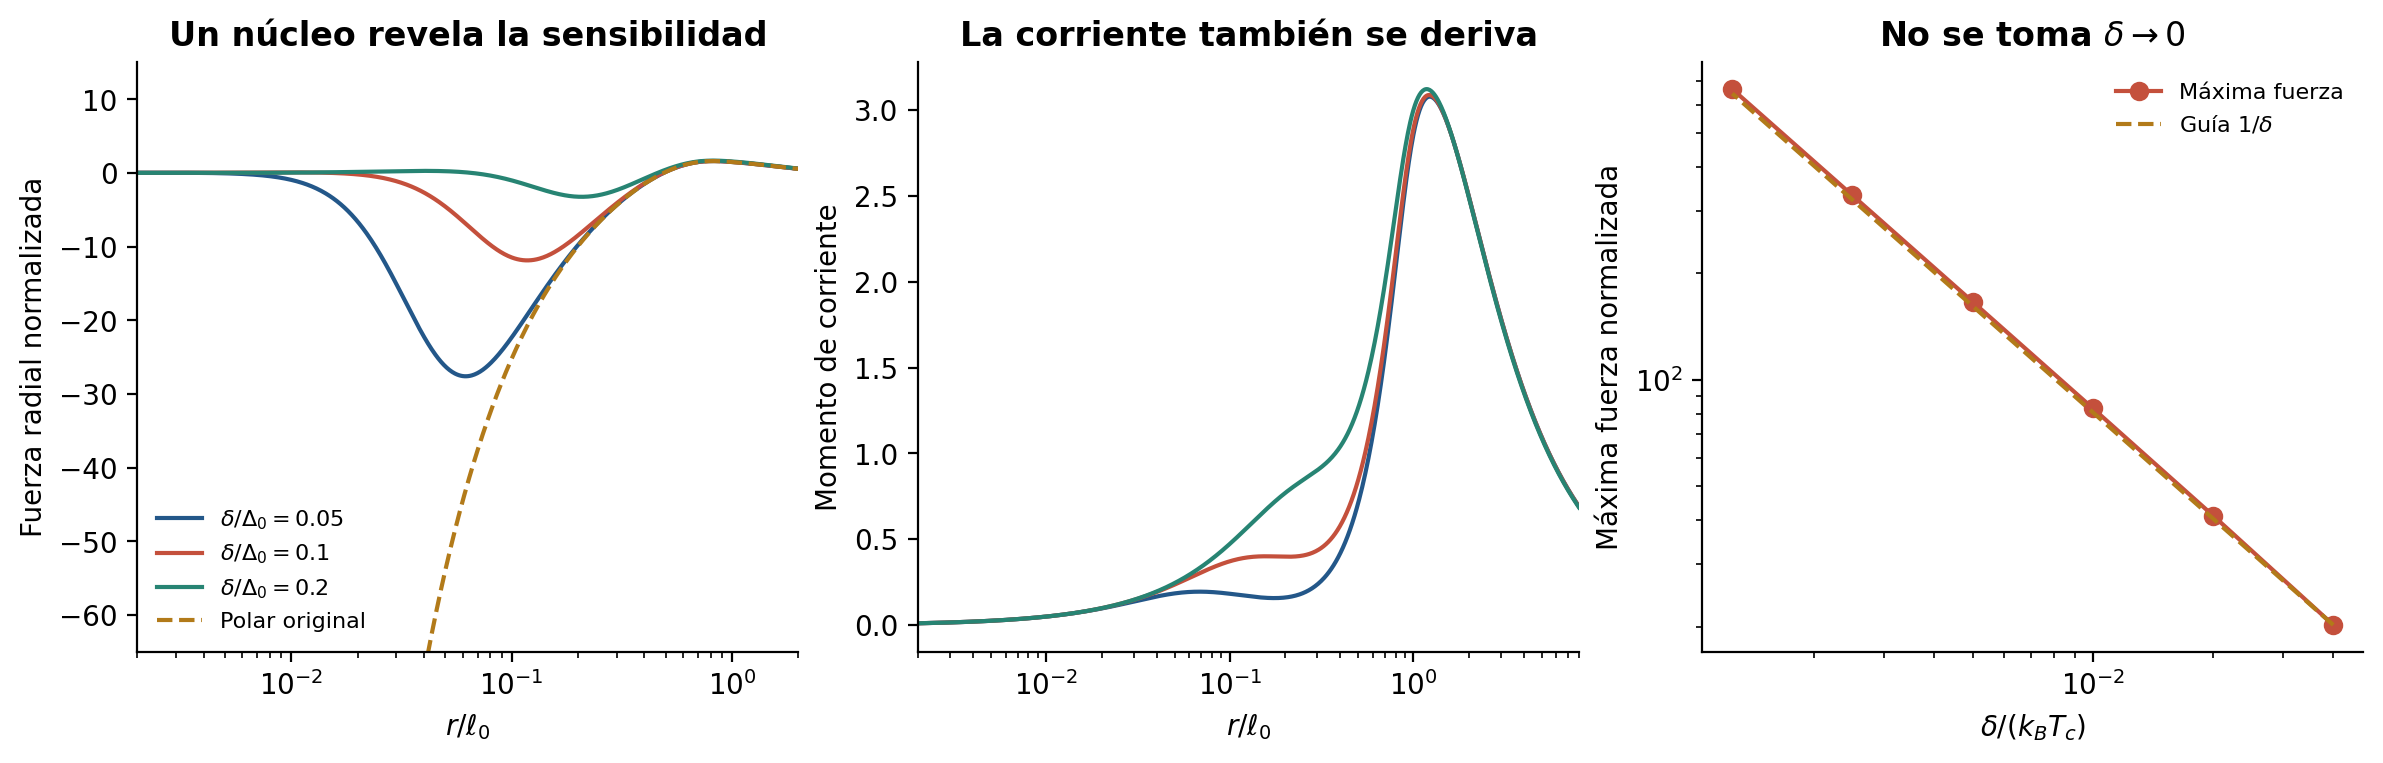
\includegraphics[width=1\linewidth,height=\textheight,keepaspectratio,alt={Figura C.1. Auditoría del núcleo. La fuerza depende fuertemente de la escala finita aunque la energía integrada varíe poco. La corriente de cada curva se deriva de la misma energía. El panel derecho muestra que forzar el regulador a cero aumenta la fuerza aproximadamente como su inversa; esa extrapolación no forma parte del modelo seleccionado.}]{../figuras/C_05_auditoria_nucleo.png}
\caption{Figura C.1. Auditoría del núcleo. La fuerza depende fuertemente
de la escala finita aunque la energía integrada varíe poco. La corriente
de cada curva se deriva de la misma energía. El panel derecho muestra
que forzar el regulador a cero aumenta la fuerza aproximadamente como su
inversa; esa extrapolación no forma parte del modelo seleccionado.}
\end{figure}

{\def\LTcaptype{none} % do not increment counter
\begin{longtable}[]{@{}
  >{\raggedleft\arraybackslash}p{(\linewidth - 6\tabcolsep) * \real{0.2500}}
  >{\raggedleft\arraybackslash}p{(\linewidth - 6\tabcolsep) * \real{0.2500}}
  >{\raggedleft\arraybackslash}p{(\linewidth - 6\tabcolsep) * \real{0.2500}}
  >{\raggedleft\arraybackslash}p{(\linewidth - 6\tabcolsep) * \real{0.2500}}@{}}
\toprule\noalign{}
\begin{minipage}[b]{\linewidth}\raggedleft
\(\delta/\Delta_0\)
\end{minipage} & \begin{minipage}[b]{\linewidth}\raggedleft
Energía excedente normalizada
\end{minipage} & \begin{minipage}[b]{\linewidth}\raggedleft
Máxima fuerza radial absoluta
\end{minipage} & \begin{minipage}[b]{\linewidth}\raggedleft
Radio de ese máximo, en \(\ell_0\)
\end{minipage} \\
\midrule\noalign{}
\endhead
\bottomrule\noalign{}
\endlastfoot
0.05 & 45.8601 & 27.6104 & 0.0615 \\
0.10 & 46.0937 & 11.8815 & 0.1180 \\
0.20 & 46.4402 & 3.2513 & 0.2073 \\
\end{longtable}
}

La energía se expresa por unidad de espesor en \(N_0(k_BT_c)^2\ell_0^2\)
y la fuerza en \(N_0k_BT_c\). La dispersión de energías dividida por la
referencia central es \textbf{1.26\%}, pero la de fuerzas máximas es
\textbf{205\%}. Reducir \(\delta\) de \(0.04k_BT_c\) a \(0.00125k_BT_c\)
en la prueba lineal del centro aumenta la fuerza máxima de 20.2 a 665.6,
aun cuando la energía converge.

\textbf{Decisión:} se conserva C.9 con \(\delta=0.10\Delta_0\) sólo como
contrato experimental cerrado para desarrollar y verificar el
acoplamiento. La prueba rechaza que esa regularización esté físicamente
validada para nucleación, vórtices o tiempos de detección. Antes de
promoverla se necesita una referencia espacial y comprobar observables
de núcleo; conservar energía con precisión no sustituye esa comparación.
No se propone implementar un Usadel espacial no térmico completo sin
resolver también su compatibilidad con B.

\section{C.8. Una prueba espacial que anticipa errores de
relajación}\label{c.8.-una-prueba-espacial-que-anticipa-errores-de-relajaciuxf3n}

Un segundo diagnóstico evita el núcleo y pregunta por pequeñas
modulaciones de amplitud alrededor del estado uniforme térmico, a
\(q=0\). En unidades \(k_BT_c\) y \(\ell_0\), sea
\(d=|\Delta|/(k_BT_c)\), \(\epsilon_n=\pi(T/T_c)(2n+1)\) y
\(E_n=\sqrt{\epsilon_n^2+d^2}\). La ecuación Usadel espacial linealizada
para una modulación de número de onda \(k\) da

\[
\delta\Theta_{n,k}=\frac{\epsilon_n/E_n}{E_n+(k\ell_0)^2}\,\delta d_k.
\tag{C.29}
\]

La respuesta espectral a una variación rápida en el espacio es menor que
la respuesta local \(k=0\). Al sustituirla en la fuerza de amplitud,

\[
\begin{aligned}
H_U(k)-H_U(0)
&=4\pi\frac{T}{T_c}\sum_{n\geq0}
\frac{(\epsilon_n/E_n)^2(k\ell_0)^2}{E_n[E_n+(k\ell_0)^2]},\\
H_{K_0}(k)&=H_U(0)+\frac{\pi}{2}(k\ell_0)^2.
\end{aligned}\tag{C.30}
\]

\(H\) es la derivada de la fuerza normalizada respecto de \(d\), no una
energía térmica. La segunda fila corresponde al cierre local de
gradiente que también usa C.9 para perturbaciones de amplitud a \(q=0\).
Con la \textbf{misma} movilidad KWT impuesta a ambas respuestas, el
tiempo de relajación lineal condicional es

\[
t_{\rm rel}(k)=\frac{2\sqrt{(1+T/T_c)/2}\,R\,\tau_0}{H(k)}.
\tag{C.31}
\]

\begin{figure}
\centering
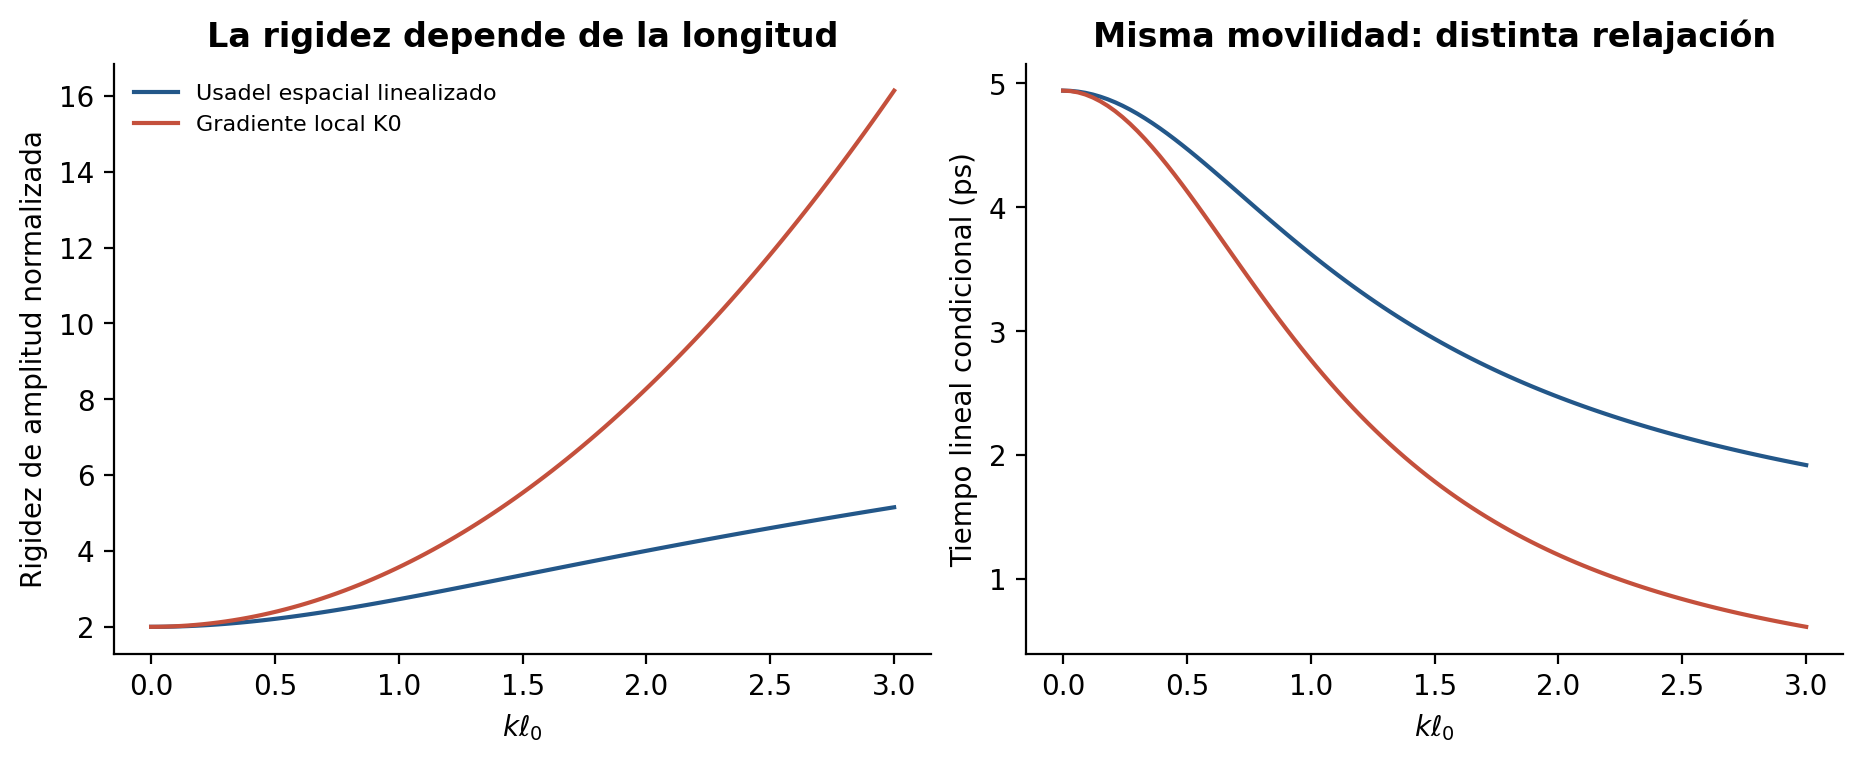
\includegraphics[width=0.96\linewidth,height=\textheight,keepaspectratio,alt={Figura C.2. Modulación infinitesimal de amplitud en un superconductor uniforme. El cierre K0 endurece las perturbaciones cortas respecto de la respuesta espacial linealizada. Al aplicar la misma movilidad, predice su relajación más rápida. Esta comparación a temperatura impuesta no incorpora la cinética acoplada de B ni valida el valor de la movilidad.}]{../figuras/C_06_modos_espaciales.png}
\caption{Figura C.2. Modulación infinitesimal de amplitud en un
superconductor uniforme. El cierre K0 endurece las perturbaciones cortas
respecto de la respuesta espacial linealizada. Al aplicar la misma
movilidad, predice su relajación más rápida. Esta comparación a
temperatura impuesta no incorpora la cinética acoplada de B ni valida el
valor de la movilidad.}
\end{figure}

{\def\LTcaptype{none} % do not increment counter
\begin{longtable}[]{@{}
  >{\raggedleft\arraybackslash}p{(\linewidth - 6\tabcolsep) * \real{0.2500}}
  >{\raggedleft\arraybackslash}p{(\linewidth - 6\tabcolsep) * \real{0.2500}}
  >{\raggedleft\arraybackslash}p{(\linewidth - 6\tabcolsep) * \real{0.2500}}
  >{\raggedleft\arraybackslash}p{(\linewidth - 6\tabcolsep) * \real{0.2500}}@{}}
\toprule\noalign{}
\begin{minipage}[b]{\linewidth}\raggedleft
\(k\ell_0\)
\end{minipage} & \begin{minipage}[b]{\linewidth}\raggedleft
Exceso de rigidez de \(K_0\)
\end{minipage} & \begin{minipage}[b]{\linewidth}\raggedleft
Tiempo con respuesta espacial
\end{minipage} & \begin{minipage}[b]{\linewidth}\raggedleft
Tiempo con gradiente \(K_0\)
\end{minipage} \\
\midrule\noalign{}
\endhead
\bottomrule\noalign{}
\endlastfoot
0.30 & 3.03\% & 4.756 ps & 4.616 ps \\
0.99 & 30.31\% & 3.639 ps & 2.793 ps \\
2.01 & 107.75\% & 2.460 ps & 1.184 ps \\
\end{longtable}
}

Pasar de 2500 a 5000 frecuencias cambia la respuesta menos de
\(4.4\times10^{-6}\) relativo. La comparación debe permanecer dentro del
régimen difusivo \(k\ell\ll1\), donde \(\ell\) es el libre recorrido
elástico; no se usa la tabla para extrapolar a longitudes atómicas. El
resultado anticipa un sesgo concreto en escalas espaciales cortas, sin
transformar esos tiempos lineales en latencias del detector.

\subsection{C.8.1. Una segunda condición: no aceptar difusión de fase
hacia
atrás}\label{c.8.1.-una-segunda-condiciuxf3n-no-aceptar-difusiuxf3n-de-fase-hacia-atruxe1s}

La regularidad en un cero y la disipación positiva no garantizan que la
ecuación espacial esté bien planteada. Para comprobarlo se congela la
amplitud y la población \(p=0\), sin imponer autoconsistencia. En las
unidades de esta sección, \(\bar q=q\ell_0\), \(\bar q_\delta=m\bar q\)
y \(d=|\Delta|/(k_BT_c)\). La integral de Matsubara a temperatura cero
puede hacerse exactamente en el régimen \(\bar q_\delta^2<d\):
escribiendo \(\epsilon=d\cot\Theta-\bar q_\delta^2\cos\Theta\),

\[
\overline\Pi_{\rm vac}
=2\bar q_\delta\int_0^\infty\sin^2\Theta\,d\epsilon
=2\bar q_\delta\int_0^{\pi/2}(d-\bar q_\delta^2\sin^3\Theta)\,d\Theta
=\pi d\bar q_\delta-\frac43\bar q_\delta^3.
\]

\(\overline\Pi\) es la derivada de la densidad energética normalizada
respecto de \(\bar q_\delta\). La curvatura longitudinal de fase del
candidato, a amplitud y ocupaciones fijas, es por tanto

\[
H_\theta=\frac{\partial^2\overline e_\delta}{\partial\bar q^2}
=m^2(\pi d-4\bar q_\delta^2)
+\frac\pi2d^2(1-m^2).
\]

Para \(d=0.60\Delta_0/(k_BT_c)=1.058326\), \(\delta=0.10\Delta_0\) y
\(\bar q=1\), se obtiene \(\bar q_\delta=0.972973\),
\(\bar q_\delta^2=0.946676<d\) y \textbf{\(H_\theta=-0.343431\)}. A
\(\bar q=0.65\), en cambio, vale \(1.726783\). La derivada se toma a
amplitud fija; no es la caída de corriente debida a seguir una rama de
gap autoconsistente. Una integración independiente de la ecuación de
Matsubara seguida de diferencias de corriente coincide en el estado
negativo a \(1.11\times10^{-12}\) absoluto; refinar de 192 a 384 nodos
cambia su momento de corriente en \(1.34\times10^{-15}\).

\begin{figure}
\centering
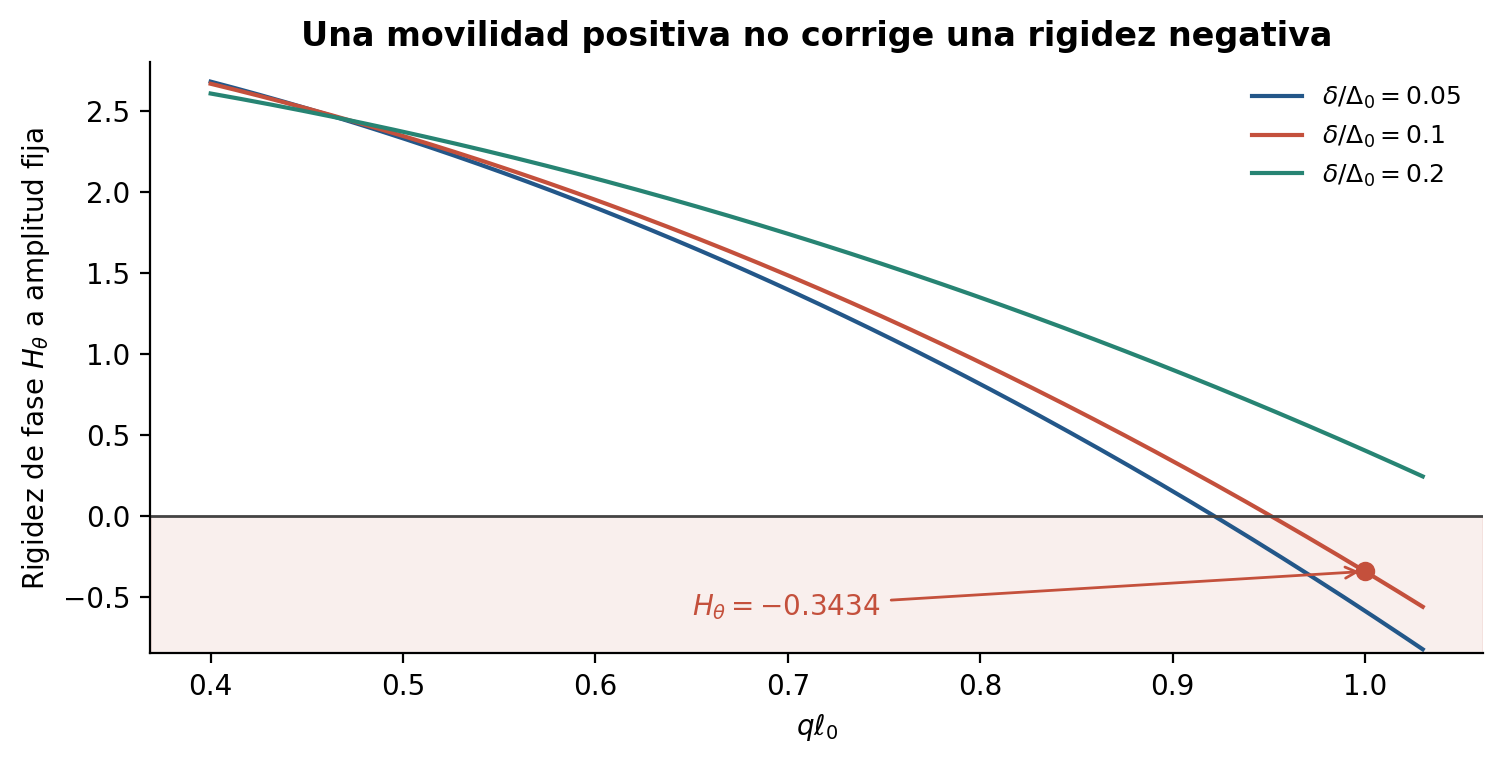
\includegraphics[width=0.96\linewidth,height=\textheight,keepaspectratio,alt={Figura C.3. Admisibilidad espacial, con amplitud fija de 0.60 Delta0 y vacío de excitaciones. Una rigidez de fase negativa permite que perturbaciones cada vez más cortas crezcan cada vez más rápido en la PDE local. Cambiar la escala de núcleo desplaza el cruce, pero no demuestra estabilidad espacial global.}]{../figuras/C_09_admisibilidad_espacial.png}
\caption{Figura C.3. Admisibilidad espacial, con amplitud fija de 0.60
Delta0 y vacío de excitaciones. Una rigidez de fase negativa permite que
perturbaciones cada vez más cortas crezcan cada vez más rápido en la PDE
local. Cambiar la escala de núcleo desplaza el cruce, pero no demuestra
estabilidad espacial global.}
\end{figure}

Con movilidad positiva, una curvatura negativa produce crecimiento
proporcional a \(k^2\) en la linealización de fase. La restricción de
Poisson añade términos de orden \(k^0\) y no elimina ese crecimiento a
número de onda grande. Interpretarlo como una nucleación calculada, o
estabilizarlo sólo con una malla gruesa, confundiría un fallo del cierre
local con física del detector.

Se fija una condición de admisión para el candidato. Con
\(\mathbf z=(\operatorname{Re}\Delta,\operatorname{Im}\Delta)\),
ocupaciones congeladas y \(\widehat{\mathbf n}\) una dirección espacial
unitaria, se evalúa

\[
M_{ab}(\widehat{\mathbf n})
=\frac{\partial^2 e_\delta}{\partial(\partial_i z_a)\,\partial(\partial_j z_b)}
\widehat n_i\widehat n_j,
\qquad \lambda_{\min}[M(\widehat{\mathbf n})]>0
\quad\text{para toda }\widehat{\mathbf n}.
\]

Esta condición se verifica antes y durante cualquier ensayo espacial. Si
se pierde, se detiene el candidato y se registra el primer estado no
admitido; no se recorta la rigidez ni se continúa atribuyendo tiempos
físicos a la trayectoria. Es una condición necesaria sobre el bloque del
condensado, no una prueba completa de existencia y estabilidad del
sistema cinético acoplado. El estado de prueba anterior queda rechazado.
No se afirma que 0.4 prediga transitorios que atraviesen ese dominio.

\section{C.9. Señal y circuito antes de
amplificación}\label{c.9.-seuxf1al-y-circuito-antes-de-amplificaciuxf3n}

Se fijan dos planos eléctricos en las continuaciones y una orientación
de izquierda a derecha:

\[
V_{\rm patch}=\int_L^R\mathbf E\cdot d\mathbf l
=\phi_L-\phi_R\quad(\mathbf A=0),\qquad
V_{\rm port}=V_{\rm patch}+L_{\rm ext}^{\rm diff}(I)\dot I.
\tag{C.32}
\]

La inductancia exterior excluye la energía ya resuelta por C.9. Para la
fuente de corriente ideal y una carga \(R_L\) en paralelo,

\[
L_{\rm ext}^{\rm diff}(I)\dot I+V_{\rm patch}=R_L(I_b-I),
\qquad V_{\rm port}=R_L(I_b-I),\qquad
\frac{dU_{\rm ext}}{dI}=I L_{\rm ext}^{\rm diff}(I).
\tag{C.33}
\]

La comprobación de potencia del circuito es

\[
\dot U_{\rm ext}+I V_{\rm patch}+R_L(I_b-I)^2=I_bV_{\rm port}.
\tag{C.34}
\]

No se añade \(LI^2/2\) a una región cuya energía de superflujo ya esté
incluida, ni se usa esa fórmula con una inductancia dependiente de
corriente sin comprobar su definición. \(V_{\rm patch}\) y
\(V_{\rm port}\) no tienen por qué alcanzar su máximo al mismo tiempo.

Las salidas previstas son ambos voltajes, \(I(t)\), balance integrado
C.21, ocupaciones, amplitud y estructura de fase. Se identifican por
separado el primer deslizamiento o vórtice, una región resistiva
transversal cuando exista y el máximo del pulso de puerto. Ninguna
prueba de esta revisión obtiene ya esos tiempos en un evento espacial
completo. La sensibilidad de C.7 impide presentar una futura trayectoria
convergida sólo en malla como predicción validada de nucleación.

\section{C.10. Trayectoria nueva de una celda BCS con
ocupaciones}\label{c.10.-trayectoria-nueva-de-una-celda-bcs-con-ocupaciones}

La prueba dinámica de 0.4 usa energía BCS real, en lugar del potencial
polinómico pedagógico de 0.3. Se conserva una celda aislada a \(q=0\),
con amplitud y ocupaciones espectrales evolucionando. En las unidades de
C.8,

\[
\begin{gathered}
E(x,d)=\sqrt{x^2+d^2},\qquad
u=d^2\left[\ln\frac{d}{d_0}-\frac12\right]+4\int Ep\,dx,\\
X=2d\ln\frac{d}{d_0}+4\int\frac{d}{E}p\,dx,
\qquad d_0=\pi e^{-\gamma_E}.
\end{gathered}\tag{C.35}
\]

Se usa la movilidad KWT declarada y se entrega \(Q_\Delta\) a la fuente
espectral efectiva seleccionada en B,

\[
\dot p=\frac{Q_\Delta\,E f_{\rm FD}(E,T_*)[1-p]}
{4\int E^2f_{\rm FD}(E,T_*)[1-p]dx},\qquad
T_*=\max(T_E,T_b),\qquad \dot u=X\dot d+Q_\Delta=0.
\tag{C.36}
\]

El factor \(N_0\) desaparece en estas unidades. Se apagan intercambio
electrón--fonón, relajación electrón--electrón, escape y trabajo
eléctrico para aislar el acoplamiento condensado--ocupaciones. La
distribución no se obliga a ser Fermi--Dirac. La prueba no pretende
describir una película aislada de sus fonones durante ese tiempo:
verifica un subsistema del modelo y muestra lo que predice bajo las
hipótesis indicadas.

\begin{figure}
\centering
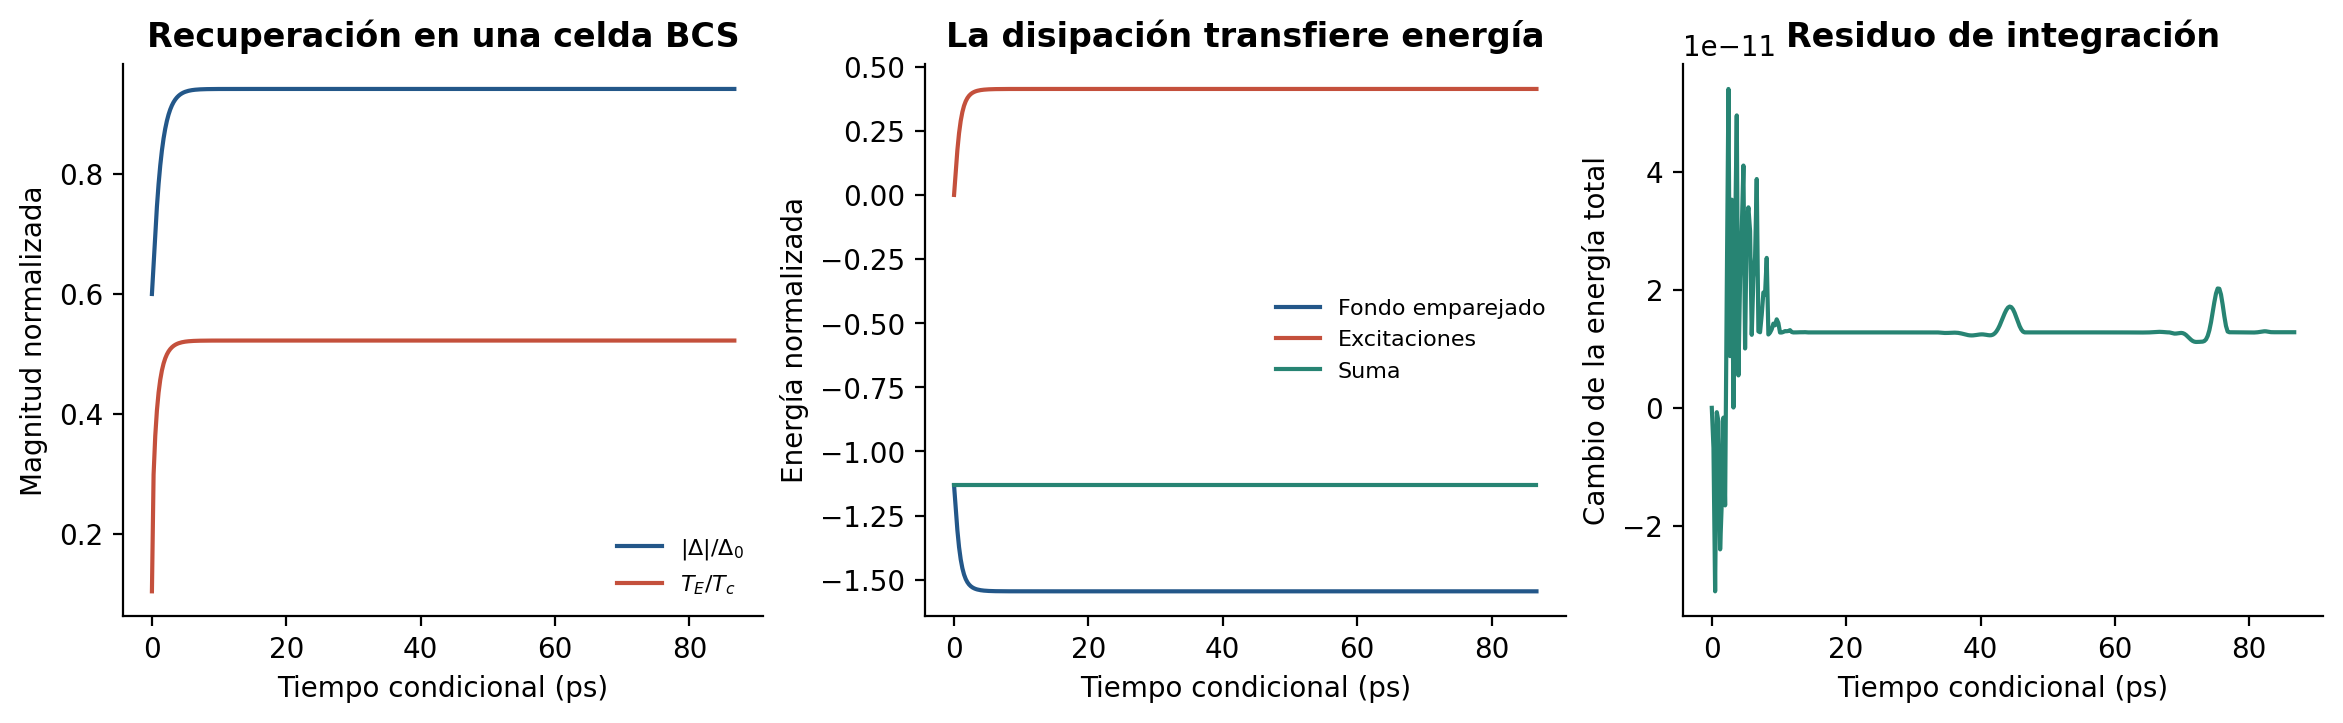
\includegraphics[width=1\linewidth,height=\textheight,keepaspectratio,alt={Figura C.4. Celda BCS aislada con poblaciones espectrales y fuente QDelta efectiva. La amplitud se recupera mientras el aumento de energía de excitaciones compensa la disminución del fondo emparejado. El último panel muestra el residuo de integración. Los tiempos dependen de la movilidad impuesta y no representan una latencia de detección.}]{../figuras/C_07_celda_BCS_cinetica.png}
\caption{Figura C.4. Celda BCS aislada con poblaciones espectrales y
fuente QDelta efectiva. La amplitud se recupera mientras el aumento de
energía de excitaciones compensa la disminución del fondo emparejado. El
último panel muestra el residuo de integración. Los tiempos dependen de
la movilidad impuesta y no representan una latencia de detección.}
\end{figure}

Se parte de \(|\Delta|=0.60\Delta_0\) y ocupaciones térmicas a 0.9 K.
Tras 86.69 ps condicionales se obtiene \(|\Delta|/\Delta_0=0.94199\) y
\(T_E=4.5182\) K. La ocupación máxima es 0.05414. La deriva de energía
normalizada es \(5.40\times10^{-11}\); refinar de 96 a 192 nodos
espectrales cambia la amplitud menos de \(1.95\times10^{-6}k_BT_c\) y
\(T_E/T_c\) menos de \(4.22\times10^{-7}\).

El cálculo muestra que el conjunto B/C puede transferir energía durante
una recuperación no lineal sin una ecuación de temperatura como variable
primaria. También evidencia su alcance: el estado final depende del
operador de calentamiento efectivo y de los canales omitidos. No valida
por separado esos operadores ni los tiempos KWT.

\section{C.11. Alcance computacional y condición de
promoción}\label{c.11.-alcance-computacional-y-condiciuxf3n-de-promociuxf3n}

El prototipo requiere por celda el campo complejo, las ocupaciones y el
catálogo espectral evaluado en \((|\Delta|,q_\delta)\). La escala finita
evita un cociente numérico de fase, pero no elimina el coste de
colisiones ni la restricción eléctrica global. Una descomposición de
coste es

\[
W\simeq W_{\rm catálogo}+N_t\left[C_{\rm campo}(N)
+c_{\rm espectro}NN_E N_\Omega\right]+W_{\rm colas}.
\tag{C.37}
\]

Los términos deben medirse con el algoritmo final. Las pruebas nuevas se
ejecutan en Geminga en segundos y no modifican el solver de producción.
Anticipan fallos de núcleo, rigidez espacial y contabilidad de un
subsistema; no permiten deducir el tiempo de un transitorio 2D ni su
latencia física.

La decisión de esta iteración es concreta: \textbf{implementar y evaluar
el contrato experimental de las ecuaciones C.8--C.24 en un entorno de
pruebas}, con los balances y fronteras de B--D y la condición de
admisión de la sección C.8.1, manteniendo producción sin cambios. La
promoción requiere resolver la sensibilidad de núcleo de C.7 y la
pérdida de parabolicidad, comparar rigideces espaciales, identificar
entradas materiales y separar movilidad KWT de relajación cinética. El
criterio no se satisface porque las pruebas algebraicas pasen.

\section{C.12. Corriente uniforme y alcance del cierre de
referencia}\label{c.12.-corriente-uniforme-y-alcance-del-cierre-de-referencia}

\subsection{C.12.1. Conservación del cierre
anterior}\label{c.12.1.-conservaciuxf3n-del-cierre-anterior}

La identidad (C.5) conserva la justificación algebraica de
Vodolazov--Allmaras: la divergencia GL del operador espacial se cancela
y queda la divergencia Usadel deseada. Esa identidad no exige que la
fuerza de amplitud antigua y la corriente deriven de una misma energía.
La sustitución (C.7) muestra qué cambia al introducirla; las ecuaciones
(C.9)--(C.13) definen su extensión finita. Así se mantiene la conexión
con la memoria sin repetir un segundo desarrollo de la misma
cancelación.

\subsection{C.12.2. La rama del prototipo se calcula con su propia
energía}\label{c.12.2.-la-rama-del-prototipo-se-calcula-con-su-propia-energuxeda}

En un estado uniforme con fase de gradiente \(q\), la densidad libre del
prototipo es

\[
f_\delta^{\rm unif}(T,|\Delta|,q)
=f_e^{\rm FD}(T,|\Delta|,mq)
+K_0|\Delta|^2q^2(1-m^2),\qquad
\partial_{|\Delta|}f_\delta^{\rm unif}=0,\qquad
j_\delta=\frac{2e}{\hbar}\partial_q f_\delta^{\rm unif}.
\tag{C.38}
\]

Al derivar en amplitud también se deriva \(m\). Omitir esa dependencia
volvería a separar la fuerza de la corriente. Sobre una rama estable en
amplitud, su máximo uniforme cumple

\[
f_{\delta,qq}^{\rm unif}
-\frac{(f_{\delta,|\Delta|q}^{\rm unif})^2}
{f_{\delta,|\Delta||\Delta|}^{\rm unif}}=0,
\qquad f_{\delta,|\Delta||\Delta|}^{\rm unif}>0.
\tag{C.39}
\]

\begin{figure}
\centering
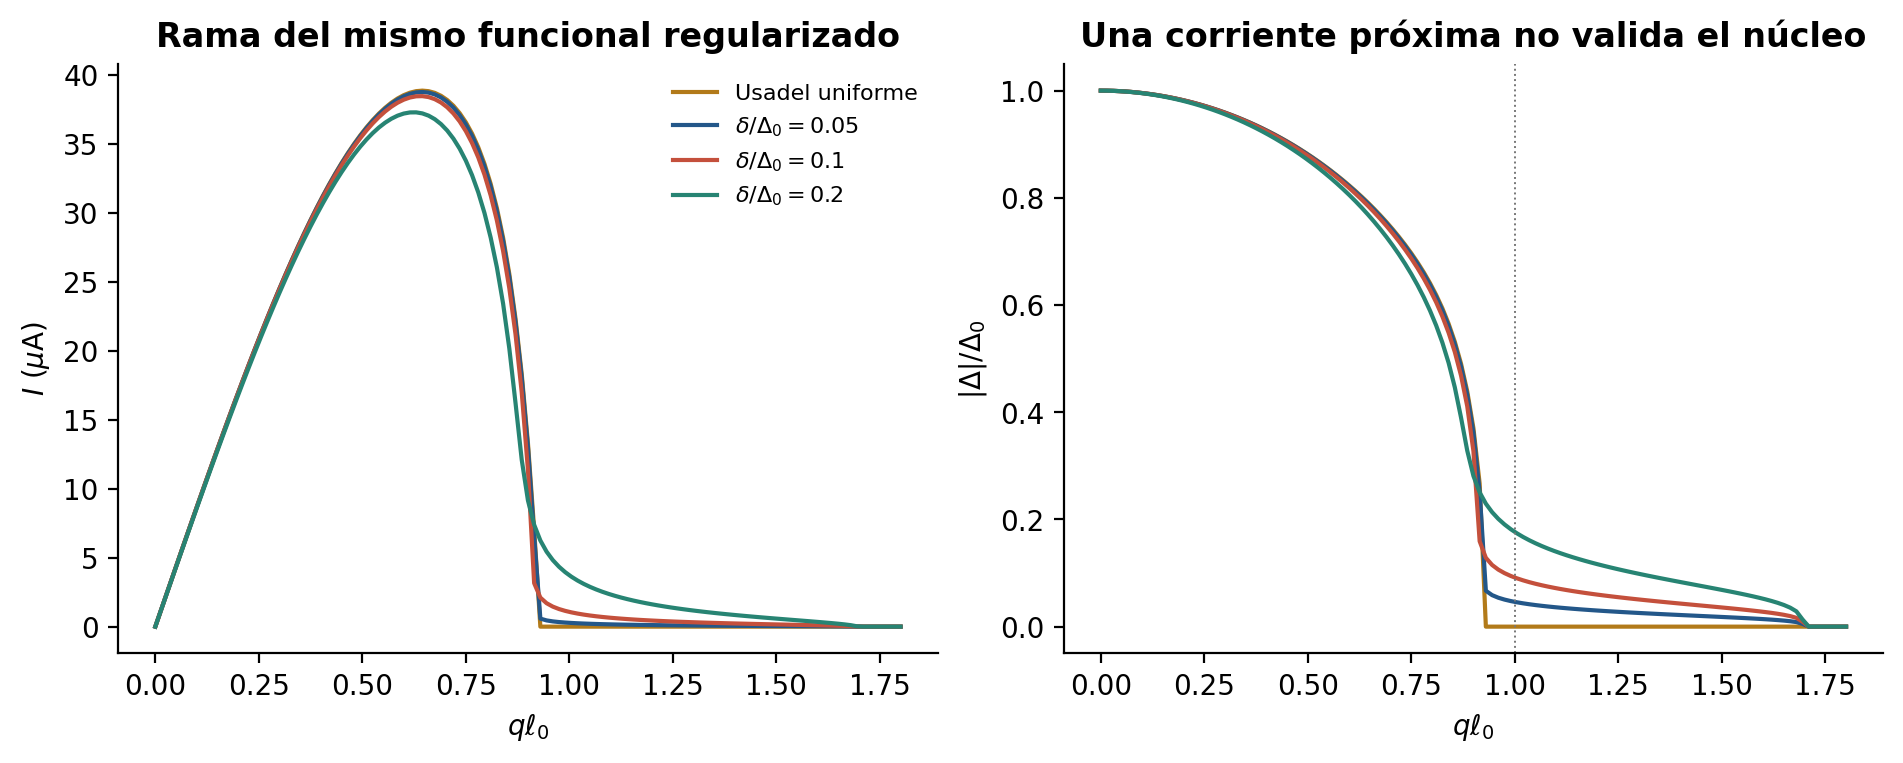
\includegraphics[width=0.96\linewidth,height=\textheight,keepaspectratio,alt={Figura C.5. Ramas uniformes de la energía regularizada y de la referencia Usadel. Todas las corrientes se derivan de la energía usada para seleccionar su amplitud. La cola de amplitud pequeña expone una modificación constitutiva del regulador que un máximo de corriente próximo puede ocultar.}]{../figuras/C_08_ramas_regularizadas.png}
\caption{Figura C.5. Ramas uniformes de la energía regularizada y de la
referencia Usadel. Todas las corrientes se derivan de la energía usada
para seleccionar su amplitud. La cola de amplitud pequeña expone una
modificación constitutiva del regulador que un máximo de corriente
próximo puede ocultar.}
\end{figure}

El barrido usa \(T=0.9\) K, \(T_c=8.65\) K, \(D=1.581\times10^{-4}\)
m\(^2\)/s, \(\sigma_n=4.2\times10^5\) S/m, ancho 120 nm y espesor 7 nm.
Para cada \(q\) se buscan ramas estacionarias positivas y se compara su
energía con el estado normal. Son parámetros de referencia compartidos
con las comprobaciones anteriores, no una nueva caracterización
material. El máximo calculado es de la rama uniforme; los bordes y
vórtices de un dispositivo pueden reducir el switching.

{\def\LTcaptype{none} % do not increment counter
\begin{longtable}[]{@{}
  >{\raggedleft\arraybackslash}p{(\linewidth - 6\tabcolsep) * \real{0.2500}}
  >{\raggedleft\arraybackslash}p{(\linewidth - 6\tabcolsep) * \real{0.2500}}
  >{\raggedleft\arraybackslash}p{(\linewidth - 6\tabcolsep) * \real{0.2500}}
  >{\raggedleft\arraybackslash}p{(\linewidth - 6\tabcolsep) * \real{0.2500}}@{}}
\toprule\noalign{}
\begin{minipage}[b]{\linewidth}\raggedleft
\(\delta/\Delta_0\)
\end{minipage} & \begin{minipage}[b]{\linewidth}\raggedleft
Máximo uniforme
\end{minipage} & \begin{minipage}[b]{\linewidth}\raggedleft
Cambio frente a Usadel
\end{minipage} & \begin{minipage}[b]{\linewidth}\raggedleft
\(|\Delta|/\Delta_0\) a \(q\ell_0=1\)
\end{minipage} \\
\midrule\noalign{}
\endhead
\bottomrule\noalign{}
\endlastfoot
0, referencia Usadel & 38.8503 \(\mu\)A & 0 & 0 \\
0.05 & 38.7520 \(\mu\)A & \(-0.2532\%\) & 0.04617 \\
0.10 & 38.4557 \(\mu\)A & \(-1.0157\%\) & 0.09157 \\
0.20 & 37.2833 \(\mu\)A & \(-4.0334\%\) & 0.17660 \\
\end{longtable}
}

La referencia elegida altera el máximo sólo un 1.02\%, pero mantiene una
amplitud pequeña en una región donde la referencia Usadel ya selecciona
el estado normal. La cola cambia aproximadamente con \(\delta\) y es un
efecto constitutivo del núcleo finito, no un error de la suma espectral.
El barrido no encontró raíces estacionarias positivas múltiples con su
resolución de búsqueda; no se usa ese hecho como prueba general de
unicidad.

La tabla numérica y la búsqueda de raíces se conservan en
\nolinkurl{C04_uniform_regularized.csv} y \nolinkurl{C04_checks.json}. La
cercanía de corrientes uniformes se interpreta junto al cambio de
fuerzas de C.7 y al de rigideces de C.8. \textbf{No se utiliza una
corriente crítica próxima para declarar resuelto el núcleo.}

\section{Referencias y procedencia}\label{referencias-y-procedencia}

{[}M{]} J. A. Díaz Monge, \emph{Multiscale Modeling of the Transient
Response of Superconducting Nanowire Single-Photon Detectors}, 2026.
Copia \nolinkurl{memoria_02.pdf}, 173 páginas: resultado complejo (C.3),
p.~impresa 121 / PDF 152; coeficientes (2.29)--(2.31), p.~31 / PDF 62;
cancelación de corriente en anexo C.2, pp.~121--123. La derivación de la
memoria se conserva; no se modifica su implementación de producción.

{[}V{]} D. Y. Vodolazov, Physical Review Applied \textbf{7}, 034014
(2017). \href{https://doi.org/10.1103/PhysRevApplied.7.034014}{DOI};
\href{https://arxiv.org/pdf/1611.06060}{preprint}. Corriente y
corrección del término de fase, pp.~10--11 del preprint; cinética
longitudinal como antecedente de B.

{[}A{]} J. P. Allmaras, \emph{Modeling and Development of
Superconducting Nanowire Single-Photon Detectors}, Caltech (2020).
\href{https://thesis.caltech.edu/13748/08/Allmaras_Thesis_Final.pdf}{PDF
oficial}. Ecuación (3.24), p.~impresa 94 / PDF 106; apéndice B.3 sobre
reformulación numérica. J. P. Allmaras et al., Physical Review Applied
\textbf{11}, 034062 (2019),
\href{https://doi.org/10.1103/PhysRevApplied.11.034062}{DOI}.

{[}F{]} P. Virtanen, A. Vargunin y M. Silaev, Physical Review B
\textbf{101}, 094507 (2020),
\href{https://doi.org/10.1103/PhysRevB.101.094507}{DOI}. El funcional
espacial difusivo, especializado en A, proporciona la referencia lineal
C.29--C.30. La extensión finita C.9 se propone aquí y no se atribuye a
ese artículo.

{[}Q{]} \nolinkurl{sandbox/model_v0_4/checks_c_v04.py}; resultados y
convergencias en \nolinkurl{verificaciones/C04_checks.json} y sus seis
CSV. Las cinco figuras de este documento proceden de cálculos
independientes de 0.4. Se distinguen variación cartesiana, perfil de
núcleo prescrito, respuesta espacial lineal, celda BCS espectral, ramas
uniformes y admisibilidad del símbolo principal. No se ejecutó un
transitorio de producción ni se usaron las tasas materiales DFT
rechazadas por la auditoría de B.

\end{document}
